\documentclass[11pt,a4paper]{article}

% Enhanced packages for better typography and layout
\usepackage[left=0.75in, right=0.75in, top=0.6in, bottom=0.6in]{geometry}
\usepackage{hyperref}
\usepackage{enumitem}
\usepackage[usenames,dvipsnames]{xcolor}
\usepackage{fontspec}
\usepackage{setspace}
\usepackage[explicit]{titlesec}
\usepackage{multicol}
\usepackage{fontawesome5}
\usepackage{graphicx} % For including images

% Modern font selection
\setmainfont{Helvetica Neue}[
    UprightFont = *-Light,
    BoldFont = *-Bold,
]
\setsansfont{Arial}

% Custom colors
\definecolor{primarycolor}{RGB}{0, 79, 159}
\definecolor{secondarycolor}{RGB}{100, 100, 100}
\definecolor{linkcolor}{RGB}{0, 112, 201}
\definecolor{headerbg}{RGB}{240, 240, 240}

% Custom section styling
\titleformat{\section}
    {\LARGE\bfseries\color{primarycolor}\sffamily}
    {}{0em}
    {#1\hrule height 0.5pt \vspace{-1em}}

\titleformat{\subsection}
    {\bfseries\color{secondarycolor}\sffamily}
    {}{0em}{#1\vspace{-0.5em}}

% Tighter space around section headings, to fit one page
\titlespacing*{\section}{0pt}{1.1em}{0.7em}
\titlespacing*{\subsection}{0pt}{0.9em}{0.4em}

% List styling
\setlist[itemize]{
    leftmargin=*,
    topsep=0.2em,
    itemsep=0.2em,
    parsep=0pt,
    label=\textbullet
}

% Hyperlink setup
\hypersetup{
    colorlinks=true,
    linkcolor=linkcolor,
    urlcolor=linkcolor,
    pdftitle={Evgeny Oleynik CV},
    pdfauthor={Evgeny Oleynik}
}

\begin{document}

% Header
\begin{center}
    \colorbox{headerbg}{\parbox{\textwidth}{
        \vspace{0.5em}
        \hspace{0.25em}
        \begin{minipage}[c]{0.2\textwidth}
            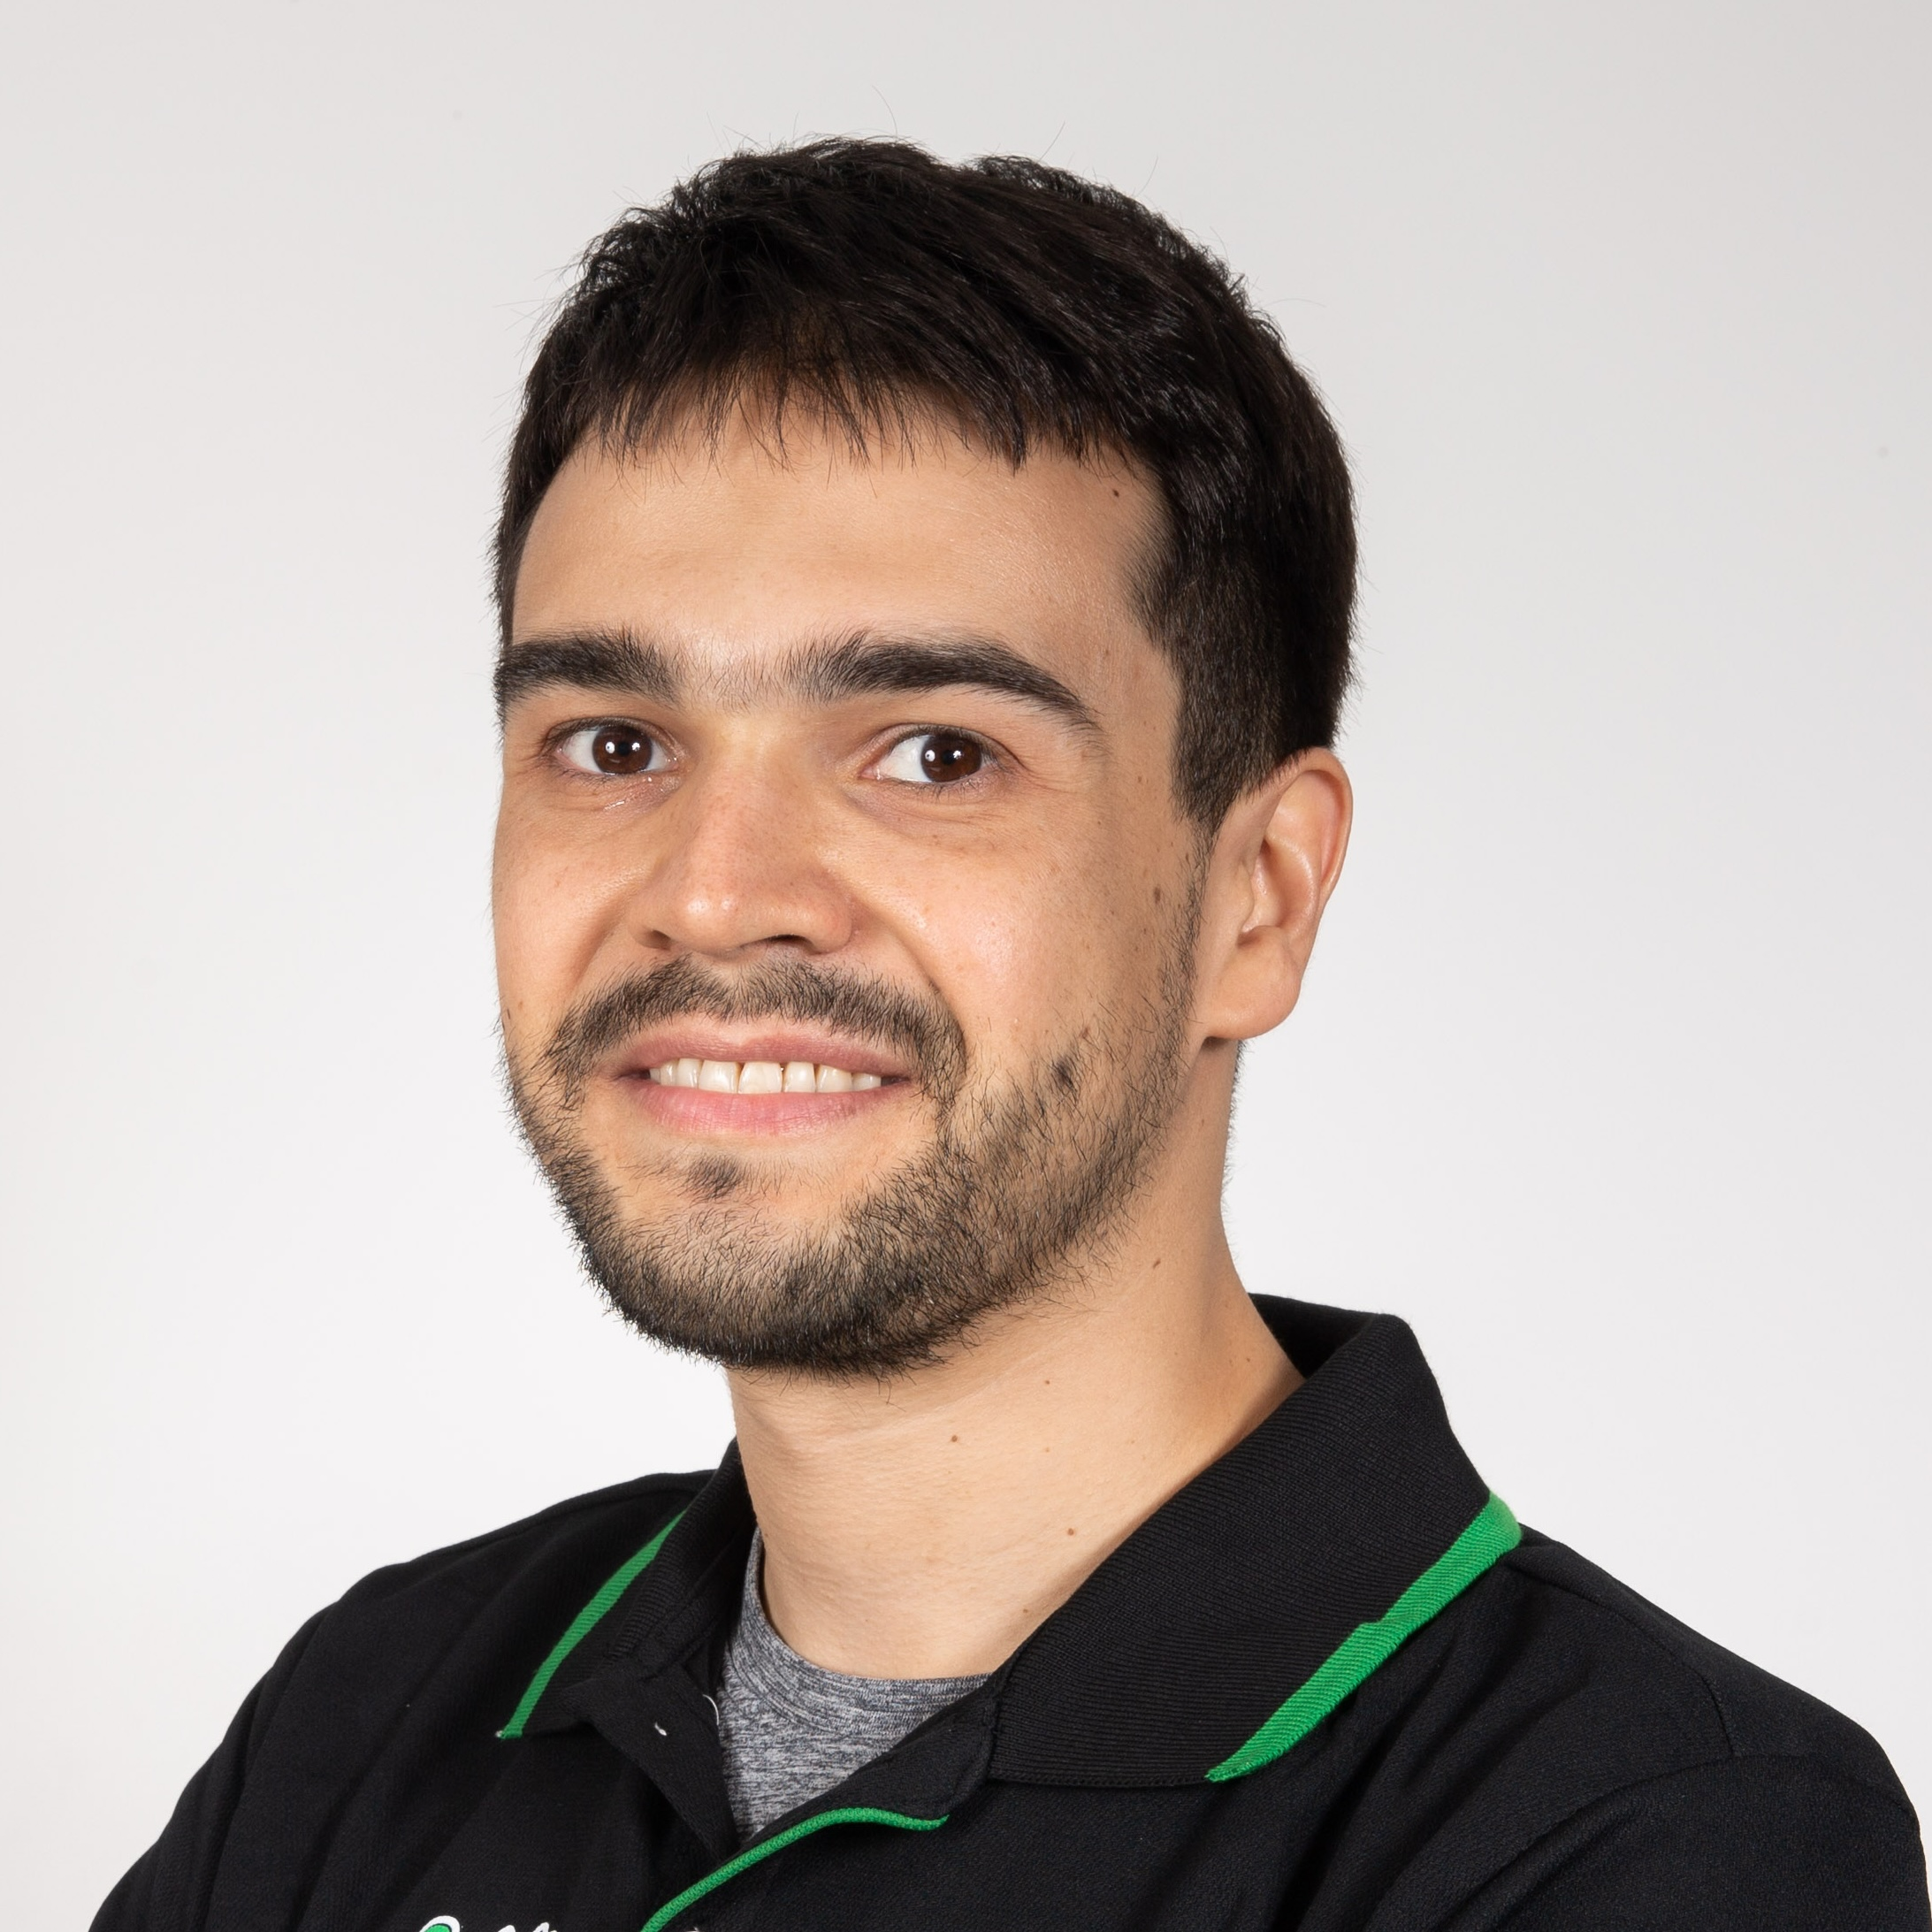
\includegraphics[width=\linewidth]{headshot.jpg} % Adjust the filename and path
        \end{minipage}\hspace{0.5em}\hfill
        \begin{minipage}[c]{0.75\textwidth}
            {\Huge\textbf{Evgeny Oleynik}} \\[0.3em]
            {\Large\color{secondarycolor} Co-Founder \& CTO, AirShelf} \\[0.5em]
            {\color{secondarycolor}
            \faMapMarker \, Singapore \\[0.2em]
            \faEnvelope \, \href{mailto:evoleinik@gmail.com}{evoleinik@gmail.com} | \faPhone \, +65 8272 3349 \\[0.2em]
            \faLinkedin \, \href{https://linkedin.com/in/evoleinik}{linkedin.com/in/evoleinik} | \faGithub \, \href{https://github.com/evoleinik}{github.com/evoleinik} | \faGlobe \, \href{https://airshelf.ai}{airshelf.ai}}
        \end{minipage}
        \vspace{0.5em}
    }}
\end{center}

% Summary
\section*{Summary}
{\setstretch{1.2}
Technical founder. Co-founder and CTO of AirShelf, an Antler-backed Singapore startup building AI sales agents for B2B sellers. Before that, ten years as co-founder and CTO of 12Go, an APAC ground transportation booking platform that connected 150+ suppliers to travellers. It grew to 50,000 bookings a day and was acquired by Bookaway (now Travelier).}

% Experience
\section*{Experience}

\subsection*{Co-Founder \& CTO \hfill Sep 2025--Present}
\textbf{AirShelf (Singapore)}
\begin{itemize}
    \item Built the product myself: an AI agent that answers B2B buyers, and their AI assistants, from the seller's own product documents. It is live on Toshiba Australia's product pages.
    \item Opened seller catalogs to AI assistants over MCP, ACP and UCP, with answers that cite their sources.
    \item Signed the first enterprise customer, Toshiba Australia, ten months after founding. Paid pilot in April 2026, annual contract in July 2026.
    \item Raised pre-seed through Antler. Selected for HP Garage and NVIDIA Inception.
\end{itemize}

\subsection*{Co-Founder \& CTO \hfill 2014--2025}
\textbf{12Go.com} \quad {\small\color{secondarycolor}\textit{Joined as senior developer, co-founder from 2015}}
\begin{itemize}
    \item Grew the platform to 50,000 bookings and \$500K GMV a day, with search at 100+ queries a second and 99.95\% uptime.
    \item Built and led a 45-person remote team across 12 departments.
    \item Designed the stack end to end: search, caching, a pricing engine over 150+ supplier integrations, and web and mobile apps. The mobile app took 30\% of bookings in its first year.
    \item Took the company through COVID-19 and led due diligence for its sale to Bookaway in 2021. My team then merged inventory, BI and finance reporting across four countries.
\end{itemize}

\subsection*{Co-Founder \& CTO \hfill 2011--2012}
\textbf{GV}
\begin{itemize}
    \item One of Southeast Asia's first holiday rental platforms. Partnered with Airbnb in Thailand.
\end{itemize}

% Skills
\section*{Skills}
\begin{itemize}
    \item \textbf{AI}: production LLM systems (Anthropic, OpenAI, Google), private GPU inference.
    \item \textbf{Engineering}: TypeScript, Next.js, PostgreSQL, AWS, Vercel.
    \item \textbf{Leadership}: hiring and running remote teams, enterprise sales, fundraising, M\&A due diligence.
\end{itemize}

% Education and languages
\section*{Education \& Languages}
Specialist degree in Applied Mathematics (MSc equivalent), Moscow Aviation Institute \hfill 2005--2010 \\[0.3em]
Russian (native), English (fluent), Thai (conversational)

\end{document}
